We illustrate this approach with an analysis of a graph from \citet{Playfair:1821}
shown in \figref{fig:playfair-wheat1}, in some ways a tour-de-force of
early graphic presentation. In this graph, Playfair used three parallel time
series in different forms
to show the price of wheat (bar chart), weekly wages (line graph), and reigning monarch (bars at the top)
over a $\sim$250 year span from 1565 to 1820. His graphic goal was rhetorical: he wished to
argue that workers had become better off in the most recent years. Surely this must be counted
among the best early data graphics.

%% one figure
\begin{figure}[htb]
  \centering
  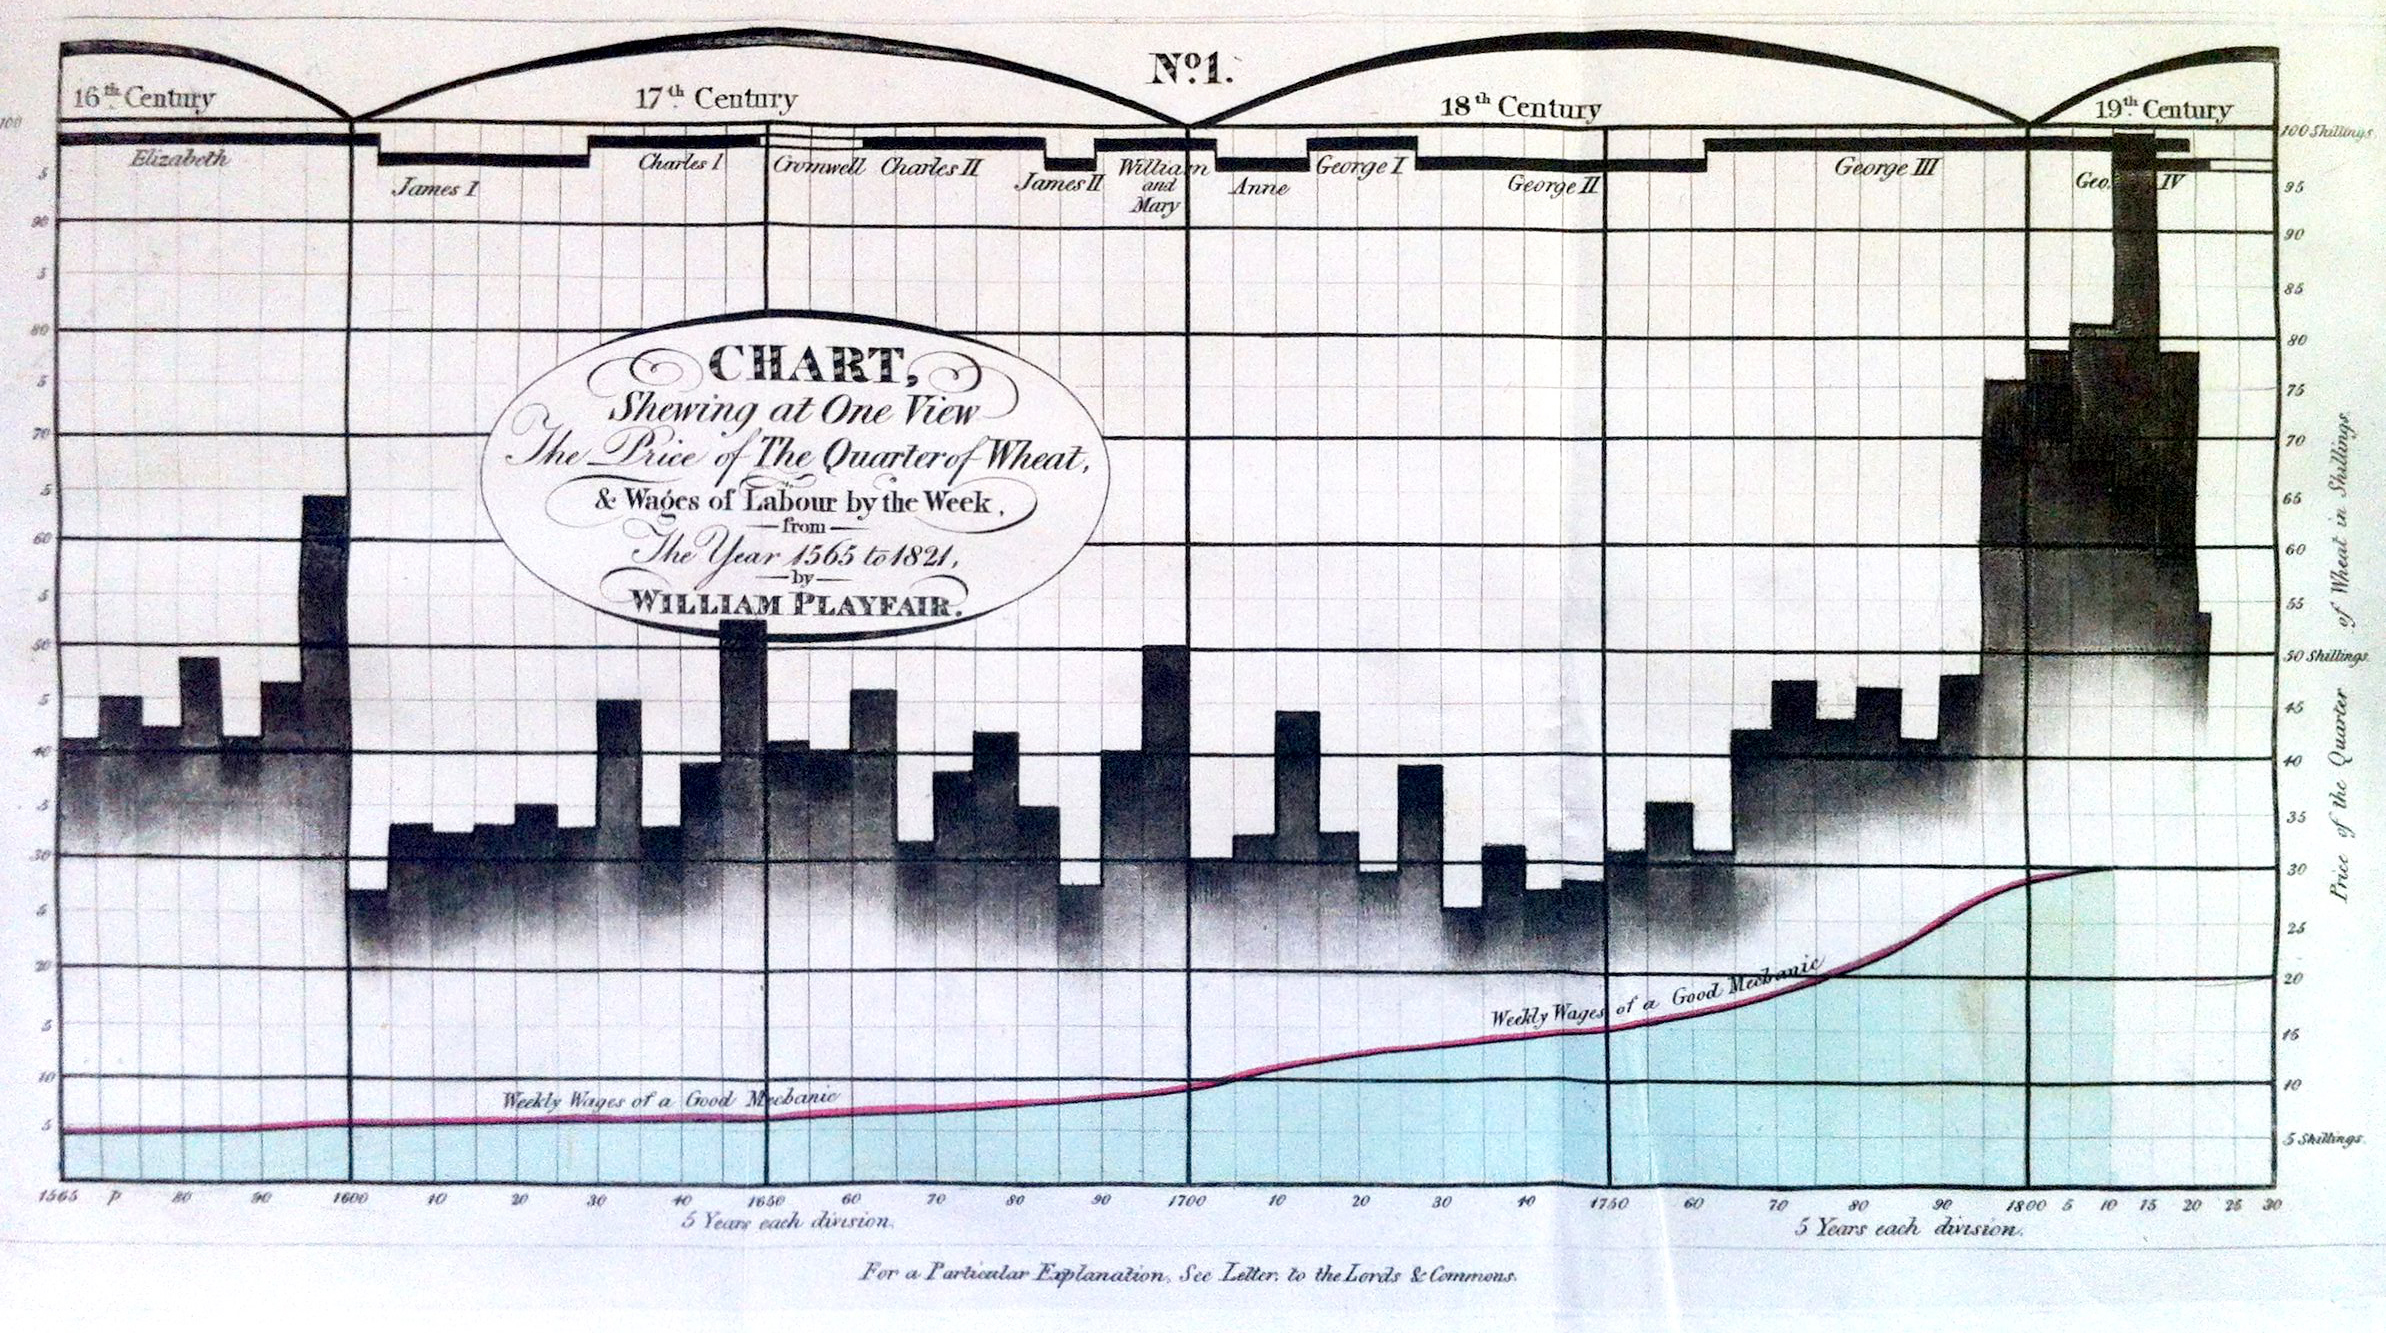
\includegraphics[width=\textwidth]{fig/Playfair1821b}
  \caption{William Playfair's 1821 time series graph of prices, wages, and ruling monarch
  over a 250 year period.
  \emph{Source}: \cite{Playfair:1821}, image from Stephen Stigler.}%
  \label{fig:playfair-wheat1}
\end{figure}

Yet, as we have argued elsewhere \citep{FriendlyDenis:05:scat}, this graph is both sinful
and a communication failure for Playfair's purpose.  It is sinful because the use of separate $y$ axes for
wages (left axis, range: 0--100) and prices (right axis, range: 0--30) on different scales
provides the opportunity to tell very different stories simply by re-scaling one or both
axes.

%% one figure
\begin{figure}[!htb]
  \centering
  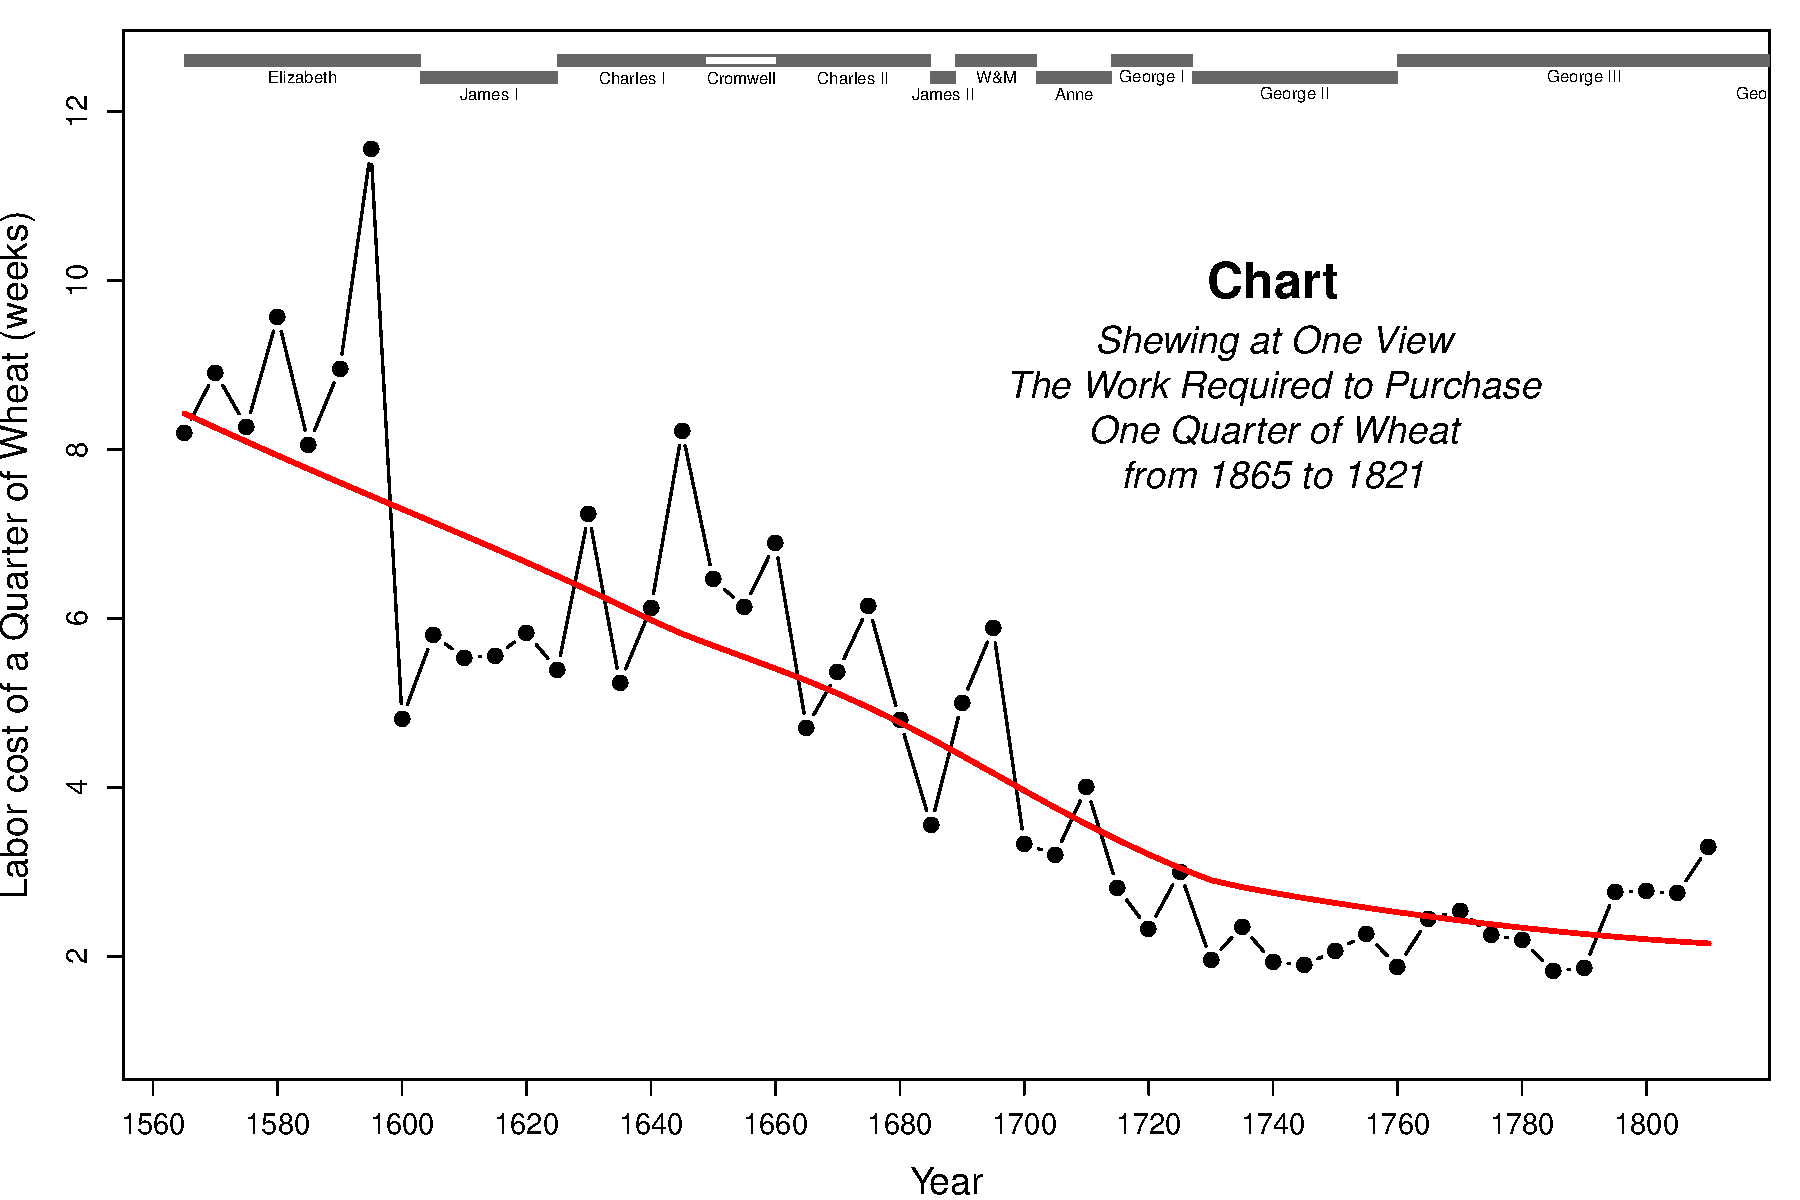
\includegraphics[width=.9\textwidth,clip]{fig/wheat2}
  \caption{Redrawn version of Playfair's time series graph
  showing the ratio of price of wheat to wages,
  together with a loess smoothed curve.}
  \label{fig:wheat1}
\end{figure}

It is also a graphic failure because the visual impression that wages increased relative to prices
toward the right end is at best indirect and is obscured by the large fluctuations in prices of wheat.
What Playfair might have done to show the relation directly, is to plot the \emph{ratio} of price to wages,
representing the labor cost of a unit of wheat, as we have done in \figref{fig:wheat1}.%
\footnote{
Playfair's data and this re-creation can be found in the \texttt{R} package HistData \citep{HistData}
as \texttt{example(Wheat)}.
}
Adding a non-parametric (loess) smoothed curve to the line plot makes Playfair's message directly apparent;
it also shows that the reduction in the amount of labor required to purchase one unit of week in fact
levels off in the last 40 years. As well, it highlights that something quite unusual happened around 1600.
